\documentclass{exam}

\usepackage{units} 
\usepackage{parskip} 
\usepackage{graphicx}
\usepackage[fleqn]{amsmath}
\usepackage{cancel}
\usepackage{float}
\usepackage{mdwlist}
\usepackage{booktabs}
\usepackage{cancel}
\usepackage{polynom}
\usepackage{caption}
\usepackage{fullpage}
\usepackage{comment}
\usepackage{enumerate}
\usepackage{xfrac}

\newcommand{\dg}{\ensuremath{^\circ}} 
\everymath{\displaystyle}

% \printanswers
\excludecomment{comment}

\ifprintanswers 
  \usepackage{2in1, lscape} 
\fi

\author{}
\date{November 6, 2013}
\title{Math 142 \\ Homework Ten}

\begin{document}

  \maketitle

  \section{Homework}
  Section 6.4: 1-8, 11-12, 17-22, 27-28, 31-38, 40-41

  \section{Extra Credit}
  Section 6.4: 42 (pretty hard)

  \ifprintanswers

  \begin{description}
    \item[41]

      There are three different triangles, and each triangle provides three equations.  Instead of writing $\sin 60$,
      $\sin A$, etc., I used $w$, $x$,$y$, for the sines of the angles.  Since all of the sines cancel out in the end,
      this works out fine.

      The equations you need are:
      \begin{align*}
        \frac{z}{a} &= \frac{x}{c + d} \\
        \frac{x}{d} &= \frac{y}{r} \\
        \frac{z}{a} &= \frac{w}{r} \\
        \frac{x}{c} &= \frac{y}{a} \\
        \frac{w}{b} &= \frac{x}{c} \\
      \end{align*}

      The procedure is:
      \begin{itemize*}
        \item solve one of the equations for a variable you want to get rid of (anything other than $a$, $b$, or
          $r$).
        \item substitute the result into the other equations
        \item repeat until you end up with an equation with $a$, $b$, and $r$
        \item solve this equation for $r$
      \end{itemize*}

      Get rid of $w$
      \begin{align*}
        \frac{w}{b} & = \frac{x}{c} \\
        w           & = \frac{xb}{c} \\
        \\
        \frac{z}{a} & = \frac{xb}{rc} \\
      \end{align*}

      The equations now are:
      \begin{align*}
        \frac{z}{a} & = \frac{x}{c + d} \\
        \frac{x}{d} & = \frac{y}{r} \\
        \frac{x}{c} & = \frac{y}{a} \\
        \frac{z}{a} & = \frac{xb}{rc} \\
      \end{align*}

      Get rid of $z$:
      \begin{align*}
        \frac{z}{a}     & = \frac{xb}{rc} \\
        z               & = \frac{abx}{rc} \\
        \\
        \frac{z}{a}     & = \frac{x}{c + d} \\
        \frac{abx}{arc} & = \frac{x}{c + d} \\
        \frac{b}{rc}    & = \frac{1}{c + d} \\
      \end{align*}

      The equations now are:
      \begin{align*}
        \frac{b}{rc} & = \frac{1}{c + d} \\
        \frac{x}{d}  & = \frac{y}{r} \\
        \frac{x}{c}  & = \frac{y}{a} \\
      \end{align*}

      Get rid of $d$:
      \begin{align*}
        \frac{x}{d}  & = \frac{y}{r} \\
        d            & = \frac{xr}{y} \\
        \\
        \frac{b}{rc} & = \frac{1}{c + \sfrac{xr}{y}} \\
        \frac{b}{rc} & = \frac{y}{yc + xr} \\
      \end{align*}

      The equations now are:
      \begin{align*}
        \frac{x}{c}  & = \frac{y}{a} \\
        \frac{b}{rc} & = \frac{y}{yc + xr} \\
      \end{align*}

      Get rid of $y$:
      \begin{align*}
        \frac{x}{c}  & = \frac{y}{a} \\
        y            & = \frac{xa}{c} \\
        \\
        \frac{b}{rc} & = \frac{y}{yc + xr} \\
        \frac{b}{rc} & = \frac{xa}{c(xa + xr)} \\
      \end{align*}

      $x$ and $c$ both cancel:
      \begin{align*}
        \frac{b}{rc} & = \frac{xa}{c(xa + xr)} \\
        \frac{b}{r} & = \frac{xa}{x(a + r)} \\
        \frac{b}{r}  & = \frac{a}{a + r} \\
      \end{align*}

      solve for $r$:
      \begin{align*}
        \frac{b}{r} & = \frac{a}{a + r} \\
        b(a + r)    & = ra \\
        ab + rb     & = ra \\
        ra - rb     & = ab \\
        r           & = \frac{ab}{a - b} \\
      \end{align*}
  \end{description}

  \fi

  \section{Review}

  \begin{enumerate}
    \item A bike with 26 inch diameter wheels is traveling at 15 mph.  What is the RPM for the wheels?

    \item Find an equation for this graph:
      \begin{figure}[h]
        \centering
        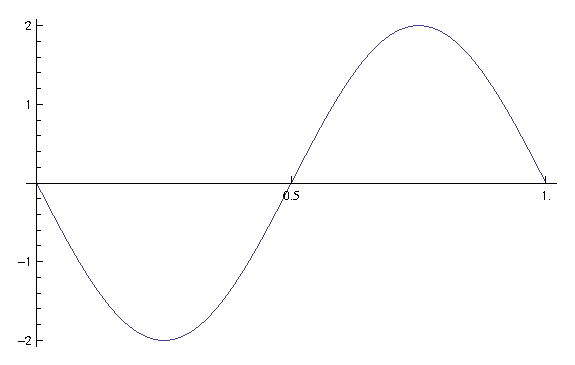
\includegraphics[scale=0.7]{review.eps}
        \caption{Find the Equation}
      \end{figure}

      \begin{solution}
        \[
          f(t) = -2 \sin 2 \pi t
        \]
      \end{solution}

  \end{enumerate}
  
  \ifprintanswers

    \section{Section 6.4}

    \begin{description}

      \item[1] 
        \begin{align*}
          \frac{\sin 98.4 \dg}{376} & = \frac{\sin 57 \dg}{x} \\
          x                         & \approx \boxed{ 318.8 } \\
        \end{align*}

      \item[2] 
        \begin{align*}
          \frac{\sin 37.5 \dg}{17} & = \frac{\sin 114.4 \dg}{x} \\
          x                        & \approx \boxed{ 25.43 } \\
        \end{align*}

      \item[3] 
        \begin{align*}
          \frac{\sin 58 \dg}{26.7} & = \frac{\sin 52 \dg}{x} \\
          x                         & \approx \boxed{ 24.81 } \\
        \end{align*}

      \item[4] 
        \begin{align*}
          \frac{\sin 67 \dg}{80.2} & = \frac{\sin \theta \dg}{56.3} \\
          \sin \theta              & \approx 0.6462 \\
          \theta                   & \approx \boxed{ 40.25 \dg } \\
        \end{align*}

      \item[5] 
        \begin{align*}
          \frac{\sin 120 \dg}{45} & = \frac{\sin \theta \dg}{36} \\
          \sin \theta             & \approx 0.6928 \\
          \theta                  & \approx \boxed{ 43.85 \dg } \\
        \end{align*}

      \item[6] 
        \begin{align*}
          \frac{\sin 102 \dg}{185} & = \frac{\sin 50 \dg}{x} \\
          x                        & \approx \boxed{ 144.9 } \\
        \end{align*}

      \item[7] 
        \begin{align*}
          \frac{\sin 114 \dg}{65} & = \frac{\sin 20 \dg}{b} \\
          b                       & \approx \boxed{ 24.33 } \\
          \\
          \frac{\sin 114 \dg}{65} & = \frac{\sin 46 \dg}{a} \\
          a                       & \approx \boxed{ 51.18 } \\
        \end{align*}

      \item[8] 
        \begin{align*}
          \frac{\sin 50 \dg}{2} & = \frac{\sin 30 \dg}{a} \\
          a                       & \approx \boxed{ 1.305 } \\
          \\
          \frac{\sin 50 \dg}{2} & = \frac{\sin 100 \dg}{c} \\
          c                       & \approx \boxed{ 2.571 } \\
        \end{align*}

      \item[11] 
        \begin{align*}
          \frac{\sin 62 \dg}{230} & = \frac{\sin 50 \dg}{a} \\
          a                       & \approx \boxed{ 199.5 } \\
          \\
          \frac{\sin 62 \dg}{230} & = \frac{\sin 68 \dg}{b} \\
          b                       & \approx \boxed{ 231.5 } \\
        \end{align*}

      \item[12] 
        \begin{align*}
          \frac{\sin 47 \dg}{50} & = \frac{\sin 23 \dg}{a} \\
          a                      & \approx \boxed{ 63.39 } \\
          \\
          \frac{\sin 47 \dg}{50} & = \frac{\sin 110 \dg}{b} \\
          b                       & \approx \boxed{ 64.24 } \\
        \end{align*}

      \item[17] 
        \begin{align*}
          \frac{\sin 110 \dg}{28} & = \frac{\sin B}{15} \\
          B                       & \approx \boxed{ 30 \dg } \\
          \\
          C & = 180 \dg - 110 \dg - 30 \dg \\
            & = \boxed{ 40 \dg } \\
          \\
          \frac{\sin 110 \dg}{28} & = \frac{\sin 40 \dg}{c} \\
          c                       & \approx \boxed{ 19.1 } \\
        \end{align*}

      \item[18] 
        \begin{align*}
          \frac{\sin 37 \dg}{30} & = \frac{\sin C}{40} \\
          C                      & \approx \boxed{ 53 \dg } \\
          \\
          B & = 180 \dg - 37 \dg - 53 \dg \\
            & = \boxed{ 90 \dg } \\
          \\
          \frac{\sin 37 \dg}{30} & = \frac{\sin 90 \dg}{c} \\
          c                      & \approx \boxed{ 49.8 } \\
        \end{align*}

      \item[19] 
        \begin{align*}
          \frac{\sin 125 \dg}{20} & = \frac{\sin C}{45} \\
          \sin C                  & \approx 1.84 \\
        \end{align*}

        No solution

      \item[20] 
        \begin{align*}
          \frac{\sin 38 \dg}{42} & = \frac{\sin B}{45} \\
          B                      & \approx \boxed{ 41 \dg } \\
          \\
          C & = 180 \dg - 38 \dg - 41 \dg 
            & = \boxed{ 101 \dg } \\
          \\
          \frac{\sin 38 \dg}{42} & = \frac{\sin 101 \dg}{c} \\
          c                      & \approx \boxed{ 67.0 } \\
        \end{align*}

      \item[21] 
        solution 1:
        \begin{align*}
          \frac{\sin 25 \dg}{25} & = \frac{\sin C}{30} \\
          C                      & \approx \boxed{ 30 \dg } \\
          \\
          B & = 180 \dg - 25 \dg - 30 \dg \\
            & = \boxed{ 125 \dg } \\
          \\
          \frac{\sin 25 \dg}{25} & = \frac{\sin 125}{b} \\
          b                      & \approx \boxed{ 48.4 } \\
        \end{align*}

        solution 2:
        \begin{align*}
          \frac{\sin 25 \dg}{25} & = \frac{\sin C}{30} \\
          C                      & \approx \boxed{ 150 \dg } \\
          \\
          B & = 180 \dg - 25 \dg - 150 \dg \\
            & = \boxed{ 5 \dg } \\
          \\
          \frac{\sin 25 \dg}{25} & = \frac{\sin 5 \dg}{b} \\
          b                      & \approx \boxed{ 5.1 } \\
        \end{align*}

      \item[22] 
        solution 1:
        \begin{align*}
          \frac{\sin 30 \dg}{75} & = \frac{\sin B}{100} \\
          B                      & \approx \boxed{ 42 \dg } \\
          \\
          C & = 180 \dg - 30 \dg - 42 \dg \\
            & = \boxed{ 108 \dg } \\
          \\
          \frac{\sin 30 \dg}{75} & = \frac{\sin 108 \dg}{c} \\
          c                      & \approx \boxed{ 142.7 } \\
        \end{align*}

        solution 2:
        \begin{align*}
          \frac{\sin 30 \dg}{75} & = \frac{\sin B}{100} \\
          B                      & 180 \dg - 42 \dg \\
                                 & \approx \boxed{ 138 \dg } \\
          \\
          C & = 180 \dg - 30 \dg - 138 \dg \\
            & = \boxed{ 12 \dg } \\
          \\
          \frac{\sin 30 \dg}{75} & = \frac{\sin 12 \dg}{c} \\
          c                      & \approx \boxed{ 31.2 } \\
        \end{align*}

      \item[27] 
        Find $\angle CDA$ and $\angle BDC$
        \begin{align*}
          \frac{\sin 30 \dg}{20} & = \frac{\sin CDA}{28} \\
          \angle CDA             & \approx 180 \dg - 44 \dg \\
                                 & = 136 \dg \\
          \angle BDC             & = 44 \dg \\
        \end{align*}

        Use the Law of Sines again to find $\angle CBD$
        \begin{align*}
          \frac{\sin 44 \dg}{20} & = \frac{\sin CBD}{20} \\
          \angle CBD             & \approx 44 \dg \\
        \end{align*}

        The missing angles are the third angles in the two small triangles.  You can find them by knowing that the sum
        of the angles in a triangle is $180 \dg$:
        \begin{align*}
          \angle BCD &= 180 \dg - 44 \dg - 44 \dg = \boxed{ 92 \dg } \\
          \angle DCA &= 180 \dg - 136 \dg - 30 \dg = \boxed{ 14 \dg } \\
        \end{align*}

      \item[28] 
        Since the smaller triangle on the left is an isosceles triangle, $\angle BCD = \angle CBD = 25 \dg$ 

        The third angle in this triangle is: $\angle BDC = 180 \dg - 25 \dg - 25 \dg = 130 \dg$

        Use the Law of Sines to find $BC$:
        \begin{align*}
          \frac{\sin 130 \dg}{BC} & = \frac{\sin 25 \dg}{12} \\
          \angle BC               & \approx 21.8 \\
        \end{align*}

        The third angle in the large triangle is: $\angle BAC = 180 \dg - 25 \dg - 50 \dg = 105 \dg$. 
        
        Use the Law of Sines to find $AB$:
        \begin{align*}
          \frac{\sin 105 \dg}{21.8} & = \frac{\sin 50 \dg}{AB} \\
          \angle AB                 & \approx 17.3 \\
        \end{align*}

        Now we can find the missing length:
        \[
          DA = AB - BD = 17.3 - 12 = \boxed{ 5.3 }
        \]

      \item[31] 
        \begin{parts}
          \part

            \begin{align*}
              C & = 180 \dg - 84.2 \dg - 93 \dg \\
                & = 2.8 \dg \\
              \\
              \frac{\sin 84.2 \dg}{b} & = \frac{\sin 2.8 \dg}{50} \\
              b                       & \approx \boxed{ \unit[1018]{mi} } \\
            \end{align*}

          \part
          \begin{align*}
            \sin 87 \dg & = \frac{h}{1018} \\
            h           & \approx \boxed{ \unit[1017]{mi} } \\
          \end{align*}
        \end{parts}

      \item[32] 
        \begin{parts}
          \part
            \begin{align*}
              C & = 180 \dg - 32 \dg - 48 \dg \\
                & = 100 \dg \\
              \\
              \frac{\sin 100 \dg}{5} & = \frac{\sin 48 \dg}{b} \\
              b                      & \approx \boxed{ \unit[3.77]{mi} } \\
            \end{align*}

          \part
            \begin{align*}
              \sin 32 \dg & = \frac{h}{3.77} \\
              h           & \approx \boxed{ \unit[2]{mi} } \\
            \end{align*}
        \end{parts}

      \item[33] 
        \begin{align*}
          C & = 180 \dg - 82 \dg - 52 \dg \\
            & = 46 \dg \\
          \\
          \frac{\sin 46 \dg}{200} & = \frac{\sin 52 \dg}{b} \\
          b                       & \approx \boxed{ \unit[219]{ft} } \\
        \end{align*}

      \item[34] 
        Find the other two angles:
        \begin{align*}
          \frac{\sin B}{312} & = \frac{\sin 48.6 \dg}{527} \\
          B                  & \approx 26.4 \dg \\
          C                  & = 180 \dg - 48.6 \dg - 26.4 \dg \\
                             & = 105 \dg \\
        \end{align*}

        Find $AB$
        \begin{align*}
          \frac{\sin 48.6 \dg}{527} & = \frac{\sin 105 \dg}{c} \\
          c                         & \approx \boxed{ \unit[679]{ft} } \\
        \end{align*}

      \item[35] 
        Find the third angle:
        \begin{align*}
          C & = 180 \dg - (90 \dg - 5.6 \dg) - 29.5 \dg \\
            & = 66.1 \dg \\
        \end{align*}

        Find the height
        \begin{align*}
          \frac{\sin 66.4 \dg}{105} & = \frac{\sin 29.2 \dg}{h} \\
          h                         & \approx \boxed{ \unit[56]{m} } \\
        \end{align*}

      \item[36] 
        \begin{align*}
          \frac{\sin C}{165} & = \frac{\sin 67 \dg}{180} \\
          C                  & \approx 57.54 \dg \\
          \\
          B & = 180 \dg - 67 \dg - 57.54 \dg \\
            & = 55.46 \dg \\
          \\
          \frac{\sin 55.46 \dg}{b} & = \frac{\sin 67 \dg}{180} \\
          b                        & \approx \boxed{ \unit[161]{ft} } \\
        \end{align*}

      \item[37] 
        Find the angle at the top of the tree:
        \begin{align*}
          A & = 180 \dg - 52 \dg - 90 \dg \\
            & = 38 \dg \\
        \end{align*}

        Find the height:
        \begin{align*}
          \frac{\sin 38 \dg}{215} & = \frac{\sin 30 \dg}{h} \\
          h                       & \approx \boxed{ \unit[175]{ft} } \\
        \end{align*}

      \item[38] 
        Find the angle at the top of the tower:
        \begin{align*}
          A & = 180 \dg - 58 \dg - 12 \dg - 90 \dg \\
            & = 20 \dg \\
        \end{align*}

        Find the remaining angle:
        \begin{align*}
          B & = 180 \dg - 20 \dg - 12 \dg \\
            & = 148 \dg \\
        \end{align*}

        Find the length of the wire:
        \begin{align*}
          \frac{\sin 20 \dg}{100} & = \frac{\sin 148 \dg}{a} \\
          a                       & \approx \boxed{ \unit[155]{m} } \\
        \end{align*}

      \item[40] 
        Find the angle at the top of the tower:
        \begin{align*}
          \frac{\sin 8 \dg}{30} & = \frac{\sin A}{120} \\
          A                     & \approx 33.83 \dg \\
        \end{align*}

        The angle of inclination of the hill completes a right triangle:
        \begin{align*}
          B & = 90 \dg - 33.83 \dg - 8 \dg \\
            & = \boxed{ 48.17 \dg } \\
        \end{align*}

      \item[41] 
        Find the angle between Sun-Earth-Venus
        \begin{align*}
          \frac{\sin 39.4 \dg}{0.723} & = \frac{\sin A}{1} \\
          A                     & \approx 118.61 \dg \\
        \end{align*}

        Find the remaining angle:
        \begin{align*}
          B & = 180 \dg - 118.61 \dg - 39.4 \dg \\
            & = 22 \dg \\
        \end{align*}

        Find the distance:
        \begin{align*}
          \frac{\sin 39.4 \dg}{0.723} & = \frac{\sin 22 \dg}{d} \\
          A                     & \approx \boxed{ \unit[0.4267]{AU} } \\
        \end{align*}

    \end{description}

  \else
    \vspace{1 cm}
    \begin{quote}
      \begin{em}
        As during the time of kings it would have been naive to think that the king’s firstborn son would be the fittest to
        rule, so in our time it is naive to think that the democratically elected ruler will be the fittest. The rule of
        succession is not a formula for identifying the best ruler, it is a formula for conferring legitimacy on someone or
        other and thus forestalling civil conflict.
      \end{em}
    \end{quote}
    \hspace{1.5 cm} --J.M. Coetzee (from {\em Diary of a Bad Year})
  \fi

\end{document}

